\chapter{Baggrund}
\section{Hjertet \& Kredsløb}
Hjertet, \textit{cor}, er en hul muskel, der har til opgave at pumpe blodet rundt til hele kroppen. Hjertet består af i alt fire kamre, som det kan ses på figur 3.1 nedenfor. To forkamre, atrier, og to hjertekamre, ventrikler. Atrierne fungere primært som reservoir for blod, mens ventriklerne fungerer som den effektive pumpe.\\

\begin{figure}[htb]
	\centering
	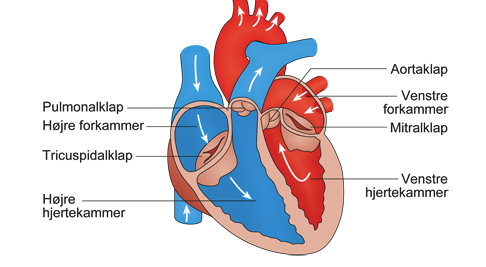
\includegraphics[width=1\textwidth]{Figurer/Fysio/Hjertet}
	\caption{Hjerte med forklarende pile \protect\cite{Hjertet}}
	\label{Hjeret} 
\end{figure}


Hjertekamrene og forkamrene er adskilt fra hinanden af anulus fibrosus, som er en plade af bindevæv. Anulus fibrosus består af fire bindevævsringe, der er forbundet med hinanden. To af disse udgør åbningerne mellem atrierne og ventriklerne. De to sidste danner åbningerne mellem højre hjertekammer og lungepulsåren og venstre ventrikel og hovedpulsåren. Ved alle bindevævsringene er der klapper, der fungere som ventiler.\\ 
AV-klapperne sidder mellem atrierne og ventriklerne. Klappen mellem højre atrium og ventrikel kaldes tricuspidalklap, mens klappen mellem venstre atrium og ventrikel kaldes mitralklap, se figur 3.1. Aortaklappen er placeret ved afgangen af hovedpulsåren og pulmonalklappen ved afgangen af lungepulsåren. Klapperne fungere således, at blodet kun kan løbe én vej gennem dem. Åbningen samt lukningen af disse er en passiv proces, som bestemmes af forskelle i væsketrykket på de to sider af klapperne.\\ 

\begin{figure}[htb]
	\centering
	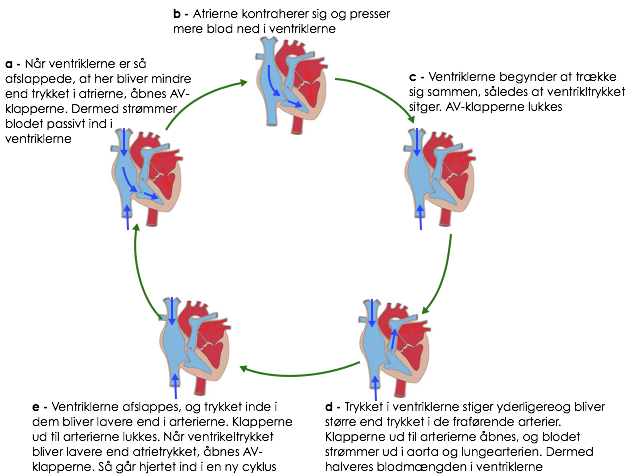
\includegraphics[width=1\textwidth]{Figurer/Fysio/Cyklus}
	\caption{De forskellige faser i hjertets cyklus \protect\cite{cyklus}}
\end{figure}

Hjertets cyklus, som er illustreret ved figur 3.2, inddeles i to hovedfaser. Den første kaldes diastolen. I diastolen er ventriklerne afslappede og fyldes med blod. Det vil sige, at trykket i ventriklerne bliver lavere end trykket i atrierne, således at AV-klapperne åbnes, og blodet begynder at strømme ind i ventriklerne. Under hele diastolen er aortaklappen lukket. Den anden fase kaldes systolen. I systolen kontraherer ventriklerne sig. Trykket i ventriklerne overstiger trykket i atrierne således, at AV-klapperne lukkes, så tilbagestrømning af blod til atrierne forhindres. Når ventriklerne har kontraheret sig så meget, at trykket i ventriklerne overstiger trykket i hovedpulsåren samt i lungepulsåren, åbnes aortaklappen og pulmonalklappen, og blodet strømmer ud i hovedpulsåren og lungepulsåren. Ventriklernes tryk falder igen til under atriernes tryk, hvilket påvirker, at AV-klapperne åbnes igen og hjertets cyklus starter forfra.\\

\section{Hæmodynamik}
Når blodet skal fra hjertet og rundt i kroppen, taler man om et blodflow. Blodets flow opfører sig som shear thinning fluid, hvilket gør sig gældende ved ikke-newtonske væsker med formindsket viskositet. At blodet hører under denne kategori, skyldes at erytrocytterne  organiseres ved et øget flow. \\
Når hjertet pumper, opstår der et tryk i blodkarrene. Blodtrykket er produktet af hjertets pumpearbejde og modstanden mod blodstrømmen i blodkredsløbet. Trykket er højest i arterierne og lavest i venerne.\cite{haemo}\\
Blodtrykket deles op i et systolisk tryk og et diastolisk tryk. Det systoliske tryk er det tryk, der opstår under hjertets sammentrækning, altså hjertets uddrivningsfase. Det diastoliske tryk opstår i hjertets afslapningsfase. I disse faser er det arterielle blodflow ikke steady, men derimod pulsatilt. 
\\Dog falder trykket ikke til 0 i diastolen pga. pulsårevæggenes elasticitet. Forholdet mellem tryk og volumen er illustreret i figur \ref{tryk og volumen}
\begin{figure}[H]
	\centering
	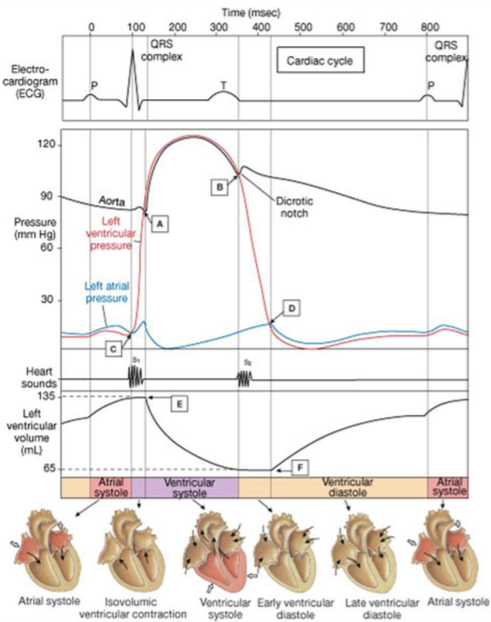
\includegraphics[width=0.8\textwidth]{Figurer/Fysio/TrykOgVolumen}
	\caption{Forhold mellem tryk og volumen\protect\cite{tryk}}
	\label{tryk og volumen}
\end{figure}
Figur \ref{tryk og volumen} viser yderligere, hvordan hjerteklappens lukning fungerer, når et trykfald herover ændrer retning. I det systemiske kredsløb er første kar aorta, som grundet sin elasticitet vil få størstedelen af blodmængden, som er pumpet ud af venstre ventrikel, til at blive dæmmet op i aorta. Dette medfører, at der oplagres en elastisk potentiel energi i aortavæggen. Denne energi udgør et tryk, der har indflydelse på og bidrager til et blodflow i diastolen efter aortaklappens lukning og hjertets uddrivningsfase. 

\section{Hypertension}
Hypertension defineres ud fra vedtagne blodtryksgrænser. De nuværende blodtryksgrænser ligger på et systolisk tryk over 140mmHg og/eller et diastolisk tryk på over 90mmHg. Disse grænserværdier gælder uanset patientens alder. Grænseværdierne er dog kun et udgangspunkt, for der kan godt opstå hypertension hos en person med et i forvejen for lavt blodtryk og i dette tilfælde vil grænseværdierne ikke nå op på værdien for definitionen af hypertension.\\
Hypertension medfører betydelig øget risiko for kardiovaskulære sygdomme, som oftest er apopleksi og iskæmisk hjertesygdom. Herudover kan hypertension medføre påvirkning af nyrerne.\cite{Hypertension}

\section{Hypotension}
Hypotension defineres som et vedvarende systolisk tryk under 100mmHg i hvile. \\
Under operationer og traumer er hypotension en mere alvorlig ting og defineres ofte som shock.\\
Shock er defineret ved en patofysiologisk tilstand karakteriseret ved, at blodcirkulationen er utilstrækkelig til at imødekomme kroppens metaboliske behov. Blodtryksgrænsen for shock angives forsimplet ofte at være systolisk blodtryk på under 90mmHg eller et fald i systolisk tryk på 40mmHg.
\cite{Hypotension}

\section{Blodtryksmåling}
For at kunne detektere et blodtryk som beskrevet i ovenstående, er det nødvendigt at foretage en blodtryksmåling. \\
Der findes mange former for blodtryksmålinger. Man skelner mellem non-invasive og invasive målinger. De non-invasive målinger kan være målemetoder som den klassiske blodtryksmåling med manchet, stetoskop og kviksølvsmanometer. Den invasive metode indebærer en indsættelse af instrument i kroppen og benyttes blandt andet på operationsstuer. Et invasivt blodtryksmålingsapparat kan deles op i to generelle metoder. Den meste brugte kliniske metode er at koble det vaskulære tryk til et eksternt sensorelement via et væskefyldt kateter. Den anden metode er en metode, hvor vandkoblingen bliver elimineret ved at inkorporere sensoren i spidsen af kateteret i det vaskulære system.\\
\\
\begin{figure}[H]
	\centering
	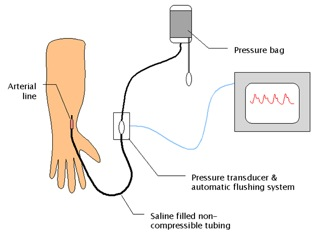
\includegraphics[width=0.6\textwidth]{Figurer/Fysio/tryk}
	\caption{Opstilling af invasiv blodtryksmåling \protect\cite{intramaaling} }
	\label{intramaaling}
\end{figure}

Som set på figur \ref{intramaaling}, placeres en nål invasivt på en patient. Nålen er forbundet til en trykpose med et natriumklorid-fyldt kateter, påsat en transducer. Posen har en udtømningsmekanisme, der sørger for, at der ikke er bobler i kateteret. Det interne tryk i posen bliver reguleret, til at ligge over patientens systoliske blodtryk. \\
Når trykket i posen reguleres, kan dette observeres på den tilkoblede monitor. Når trykreguleringen stoppes, fortsætter posen med at dryppe natriumklorid i kateteret, da det stopper blodet fra at fylde kateteret. Trykket fra patientens arterie kan nu aflæses, da trykket i kateteret stemmer overens med det tryk, der kan findes i arterien. \cite{intramaaling} 

\begin{figure}[H]
	\centering
	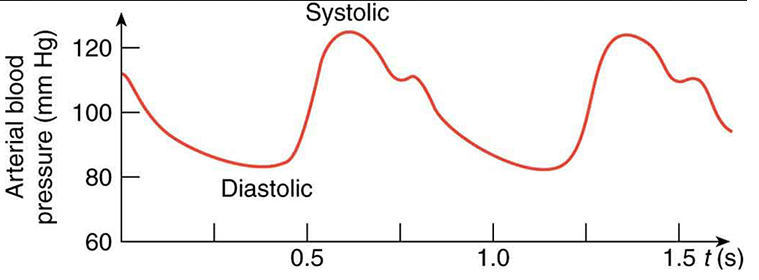
\includegraphics[width=0.6\textwidth]{Figurer/Fysio/trykmaaling}
	\caption{Grafisk afbildning af blodtryk \protect\cite{intramaalinggraf}}
	\label{grafiskmaaling}
\end{figure}

Et eksempel på en måling kan ses på figur \ref{grafiskmaaling}. Her ses det, at målingen består af en masse bølger. Disse bølger repræsenterer det samlede blodtryk, og hver bølge repræsenterer et pulslag. Toppen af bølgen repræsenterer det systoliske blodtryk, og minimum repræsenterer det diastoliske.  

\section{Sensorer}
En sensor er en transducer, der transformerer en fysisk målestørrelse til elektrisk energi. Til måling af fysiologiske størrelser som blodtryk, bruges sensorer som omformer tryk til elektrisk energi. Et eksempel på sådanne sensorer er en strain gauge som er en resistiv transducer. Strain gauges klassificeres enten som bundne eller ubundne, hvor den ubundne giver en temperaturkompensation, mens den bundne kan have udsvinging grundet temperaturen.\\
Den ubundne strain gauge består af fire sæt af strækfølsomme ledninger, der er forbundet, så de danner en Wheatstone bro, se figur \ref{StrainGauge}. Disse ledninger er monteret under tryk mellem rammen og det bevægelige armatur, således at den maksimale belastning, som strain gaugen kan holde til, er større end den forventede udefrakommende komprimerende belastning. Dette er nødvendigt for ikke at skade ledningerne. Disse typer af sensorer kan blive brugt til at konvertere blodtryk til membranbevægelse, videre til modstandsændring og til sidst et elektrisk signal. Brosammenkoblingen giver en temperaturkompensation, og den giver et fire gange så stort output fordi alle fire arme indeholder aktive gauges.\\

\begin{figure}[H]
	\centering
	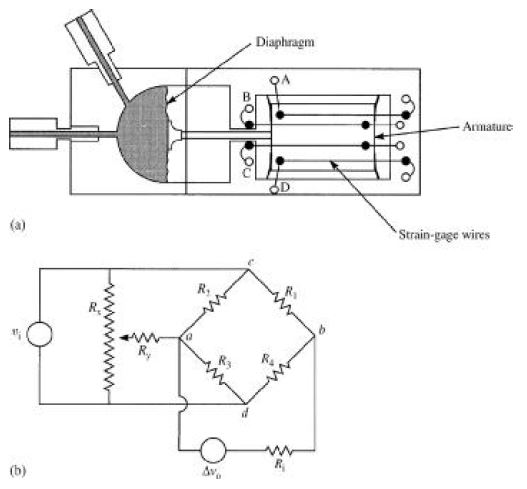
\includegraphics[width=0.6\textwidth]{Figurer/Hardware/straingauge}
	\caption{}
	\label{StrainGauge}
\end{figure}








